\section{Projekt bazy danych}
Poniższy rozdział zawiera projekt bazy danych systemu. Będzie ona przechowywała informacje o użytkownikach, grupach laboratoryjnych, stanowiskach komputerowych oraz uprawnieniach użytkowników do sal. 

Rysunek \ref{fig:diag_rel} przedstawia diagram relacyjny projektowanej bazy danych. Opis poszczególnych pól oraz ich znaczeń opisano w Tabelach \ref{tab:user_descr} (User), \ref{tab:comp_descr} (Computer), \ref{tab:classroom_descr} (Classroom), \ref{tab:croomperm_descr} (ClassroomPermission), \ref{tab:blacklist_descr} (Blacklist) oraz \ref{tab:abuse_descr} (Abuse).

\begin{figure} [!ht]
    \centering
    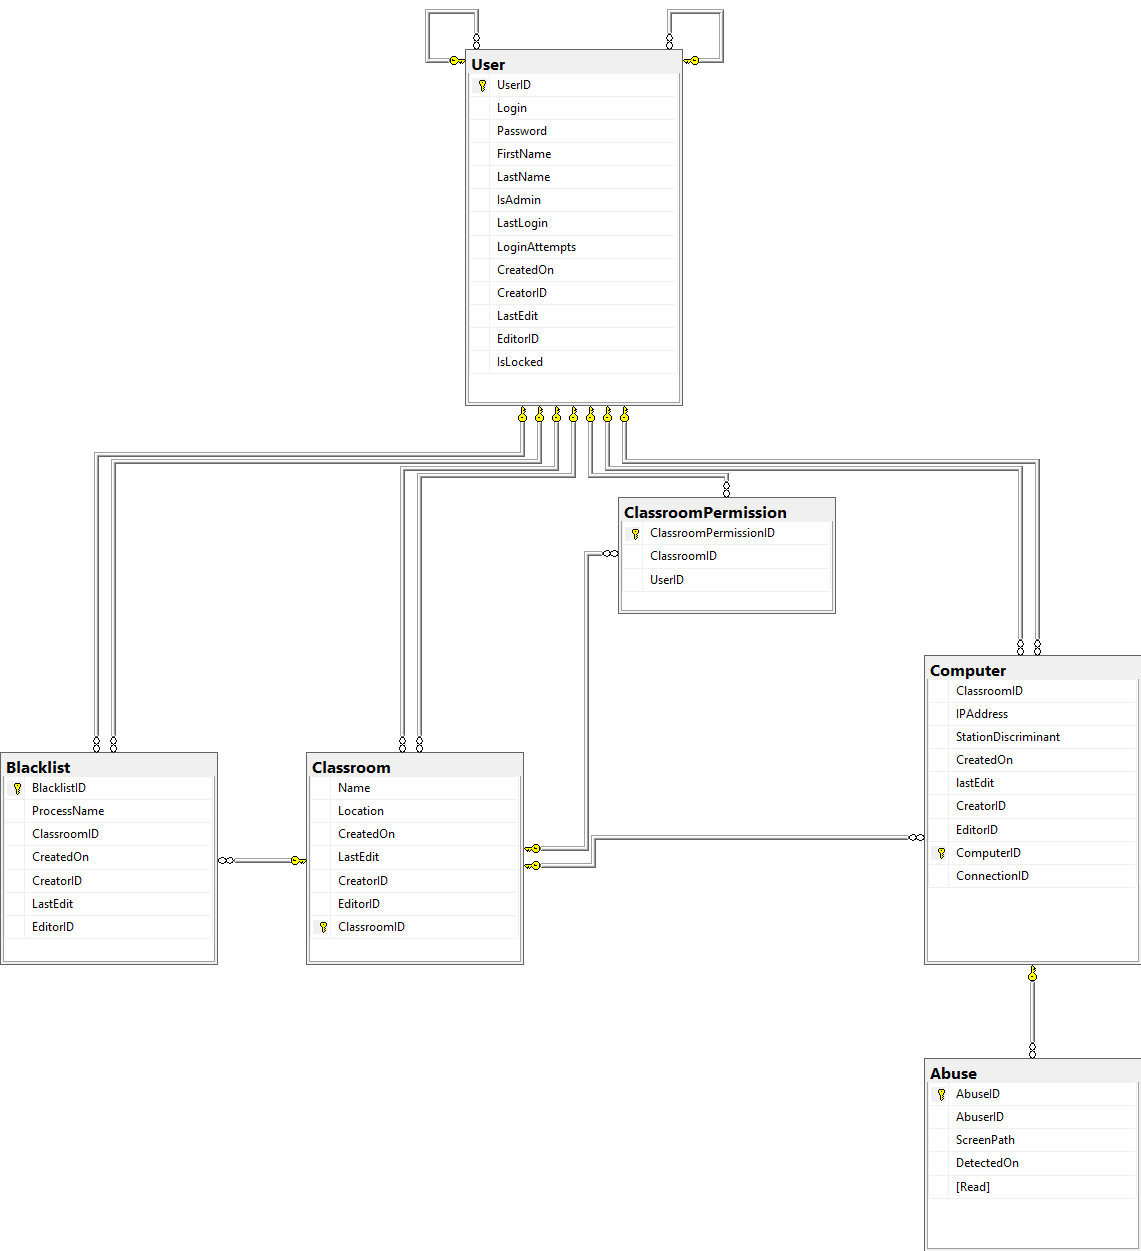
\includegraphics[height=12cm,width=15cm]{diagram_relacyjny}
    \caption{Diagram relacyjny bazy danych}
    \label{fig:diag_rel}
\end{figure}



\begin{table}[!ht]
\caption{Opis kolumn w tabeli User}
\label{tab:user_descr}
\begin{tabular}{| m{3.5cm} | m{10.5cm} |} 

\hline
Pole & Opis \\ \hline

UserID & unikatowy identyfikator użytkownika\\ \hline
Login & krótki ciąg znaków używany przez użytkowników do logowania \\ \hline 
Password & hasło do konta \\ \hline
FirstName & imię użytkownika \\ \hline
LastName & nazwisko użytkownika \\ \hline
IsAdmin & pole logiczne, którego wartość ,,Prawda'' określa, że użytkownik jest administratorem \\ \hline
LastLogin & data ostatniego poprawnego logowania do serwisu \\ \hline
LoginAttempts & licznik błędnych prób logowania \\ \hline
CreatedOn & data utworzenia użytkownika \\ \hline
CreatorID & identyfikator użytkownika, który utworzył to konto \\ \hline
LastEdit & data ostatniej edycji danych tego użytkownika \\ \hline
EditorID & identyfikator użytkownika, który ostatnio edytował dane tego konta \\ \hline
IsLocked & pole logiczne określające, czy użytkownik jest zablokowany. Gdy wartością jest prawda, użytkownik nie może się zalogować do systemu.
\\ \hline
\end{tabular}
\end{table}

\begin{table}[!ht]
\caption{Opis kolumn w tabeli Computer}
\label{tab:comp_descr}
\begin{tabular}{| m{3.5cm} | m{10.5cm} |} 

\hline
Pole & Opis \\ \hline

ID & identyfikator komputera \\ \hline
IPAdress & adres IP komputera \\ \hline
StationDiscriminant & krótki tekstowy wyróżnik\\ \hline
CreatedOn & data utworzenia tego stanowiska \\ \hline
LastEdit & data ostatniej modyfikacji danych stanowiska \\ \hline
CreatorID & identyfikator administratora, który utworzył to stanowisko \\ \hline
EditorID & identyfikator administratora, który ostatnio edytował dane tego stanowiska \\ \hline
IsConnected & oznacza, czy dany komputer jest aktualnie podłączony do serwera \\ \hline
\end{tabular}
\end{table}

\begin{table}[!ht]
\caption{\label{tab:classroom_descr}Opis kolumn w tabeli Classroom}
\begin{tabular}{| m{3.5cm} | m{10.5cm} |} 

\hline
Pole & Opis\\ \hline

ClassroomID & identyfikator sali komputerowej \\ \hline
Name & nazwa sali komputerowej  (np. jej numer)\\ \hline
Location & opis miejsca, gdzie znajduje się sala (np. budynek, piętro) \\ \hline
CreatedOn & data utworzenia sali \\ \hline
LastEdit & data ostatniej modyfikacji danych sali \\ \hline
CreatorID & identyfikator administratora, który utworzył salę \\ \hline
EditorID & identyfikator administratora, który ostatnio edytował dane sali\\ \hline
\end{tabular}
\end{table}

\begin{table}[!ht]
\caption{\label{tab:croomperm_descr}Opis kolumn w tabeli ClassroomPermission}
\begin{tabular}{| m{3.5cm} | m{10.5cm} |} 

\hline
Pole & Opis\\ \hline

ClassroomPermID & identyfikator uprawnienia do edycji danych sali \\ \hline
ClassroomID & identyfikator sali, której dotyczy to uprawnienie \\ \hline
UserID & identyfikator użytkownika, którego dotyczy to uprawnienie\\ \hline

\end{tabular}
\end{table}

\begin{table}[!ht]
\caption{\label{tab:blacklist_descr}Opis kolumn w tabeli Blacklist}
\begin{tabular}{| m{3.5cm} | m{10.5cm} |} 

\hline
Pole & Opis\\ \hline

BlacklistID & identyfikator pozycji czarnej listy \\ \hline
ProcessName & nazwa procesu niedozwolonego \\ \hline
ClassroomID & identyfikator sali, której dotyczy ta pozycja \\ \hline
CreatedOn & data utworzenia \\ \hline
LastEdit & data ostatniej modyfikacji danych czarnej listy \\ \hline
CreatorID & identyfikator administratora, który utworzył pozycję czarnej listy \\ \hline
EditorID & identyfikator administratora, który ostatnio edytował dane pozycji\\ \hline

\end{tabular}
\end{table}

\begin{table}[!ht]
\caption{\label{tab:abuse_descr}Opis kolumn w tabeli Abuse}
\begin{tabular}{| m{3.5cm} | m{10.5cm} |} 

\hline
Pole & Opis\\ \hline

AbuseID & identyfikator naruszenia \\ \hline
AbuserID & identyfikator komputera, którego dotyczy to naruszenie \\ \hline
ScreenPath & nazwa pliku ze zrzutem ekranu wykrytego naruszenia \\ \hline
DetectedOn & data i godzina wykrycia naruszenia \\ \hline

\end{tabular}
\end{table}